\subsection{K562 cell line} \label{meth-encode-k562-subsect}
After preprocessing the data, we ran EM algorithm for clustering DNA methylation profiles for the K562 cell line. As promoter regions were considered 500bp upstream and 500bp downstream of the TSS, resulting in 1000bp in total. This resulted in 5,270 promoter regions for testing. The total number of clusters K was set to 5, and the methylation profiles were modelled using $5^{th}$ degree polynomials. 

\emph{Fig. \ref{methk562:first}} depicts the five latent functions $\mathbf{f}$ (\ie clusters) that are fitted to the K562 data after running the EM algorithm. The \emph{y-axis} denotes the methylation level, and the \emph{x-axis} denotes the promoter locations scaled to the $[-1, 1]$ interval. We observe that each cluster has captured a different methylation pattern. Unsurprisingly, about 65\% of the promoter regions were assigned to cluster K=4 (\emph{red curve}), which denotes unmethylated promoter regions. The remaining four clusters had around the same percentage of assignments. From a biological viewpoint, this is expected since promoter regions of mammalian genomes are rich of CpG islands (CGIs) \citep{Illingworth2009}, which are mostly unmethylated. 

To assess the association between methylation patterns at gene promoters and gene expression, we used the corresponding RNA-Seq data to observe the expression levels of the protein-coding genes assigned to each cluster K, which are shown as \emph{boxplots} in \emph{Fig. \ref{methk562:second}}. Each coloured boxplot represents the expression level (\emph{y-axis}) of genes assigned to cluster K (\emph{x-axis}). 

Comparing the two figures we observe some functional role of the methylation patterns, which also confirm previous studies, such as \citet{Vanderkraats2013}. For example, hyper-methylation of gene promoter regions is a generally accepted mechanism for silencing gene expression. On the other hand, unmethylated promoter regions are associated with high transcription activity \citep{Deaton2011}. Finally, we observe that the U-shape of cluster K=5 (\emph{green curve}) around the TSS is also associated with higher transcription activity.
\begin{figure}[ht!]
     \begin{center}
        \subfigure[]{
            \label{methk562:first}
            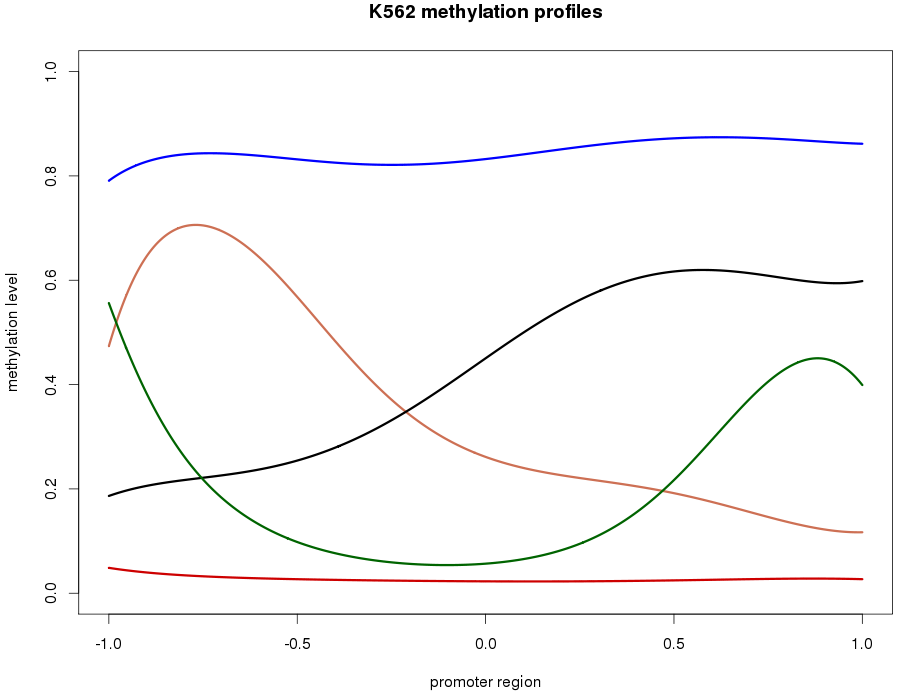
\includegraphics[width=0.45\textwidth]{images/k562MethProfClusters}
        }
        \subfigure[]{
           \label{methk562:second}
           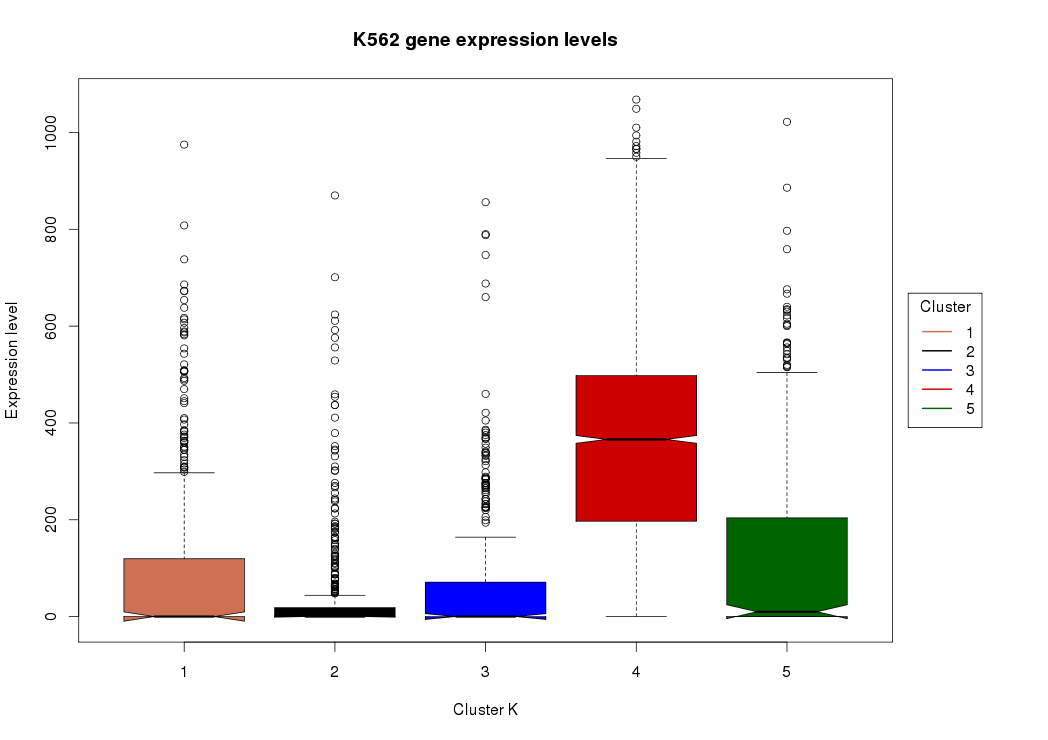
\includegraphics[width=0.495\textwidth]{images/k562MethProfBoxPlot}
        }
    \end{center}
    \caption{\emph{(a) Clustering DNA methylation profiles for the K562 cell line with $5^{th}$ degree polynomial, each colour represents a different cluster. (b) Boxplot with the corresponding gene expression levels of the protein-coding genes assigned to each cluster K for the K562 cell line. See the text for details.}}
   \label{meth-k562-pic}
\end{figure}
